\section{Auswertung}
\subsection{Vorbereitung}
Als Vorbereitung für den Verusch werden die Halbwertszeiten für $^{104}$Rh und $^{52}$V recherschiert. (Quellen: \cite{V} , \cite{Rh})
\begin{align}
    T_{^{52}\text{V}} = 224,5 \pm 0,3 \text{s}\\
    T_{^{104}\text{Rh}} = 42,3 \pm 0,4 \text{s}\\
    T_{^{104i}\text{Rh}} = 260,4 \pm 1,8 \text{s}\\
\end{align}
\subsection{Nullrate}
Über die aufgenommenen Daten für die Nullrate wurden diese Summiert und anschließend durch die Anzahl der Messwerte dividiert.
Der Mittlewert für die poissonverteilten Untergrundraten ergibt sich somit als:
\begin{align}
    N_{\text{U}} =  139\pm 4 \; \frac{\text{Imp}}{300 \text{s}} \\
    \Delta N_{\text{U}} = \sqrt{ \sum_{i=1}^n \left( \frac{1}{n}\Delta N_{\text{U}_{\text{i}}} \right)^2}
\end{align}
Mit der Anzahl $n$ der Messwerte. In diesem Experiment gilt $n = 7$.
\subsection{Vanadium}
Um mit den Berechnungen zu Beginnen muss zunächst die Untergrundrate von den messwerten abgezogen werden.
Da die Messung der Impulsrate von Vanadium in 30 Sekunden Intervallen gemacht wurde wird $N_{\text{U}}$ auf das passende Intervall angepasst.
\begin{align*}
    N_{\text{U},\text{Vanadium}} =  \frac{N_{\text{U}}}{10} = 13.9 \pm 0.4 \; \frac{\text{Imp}}{30\text{s}}
\end{align*}
\begin{figure}
    \centering
    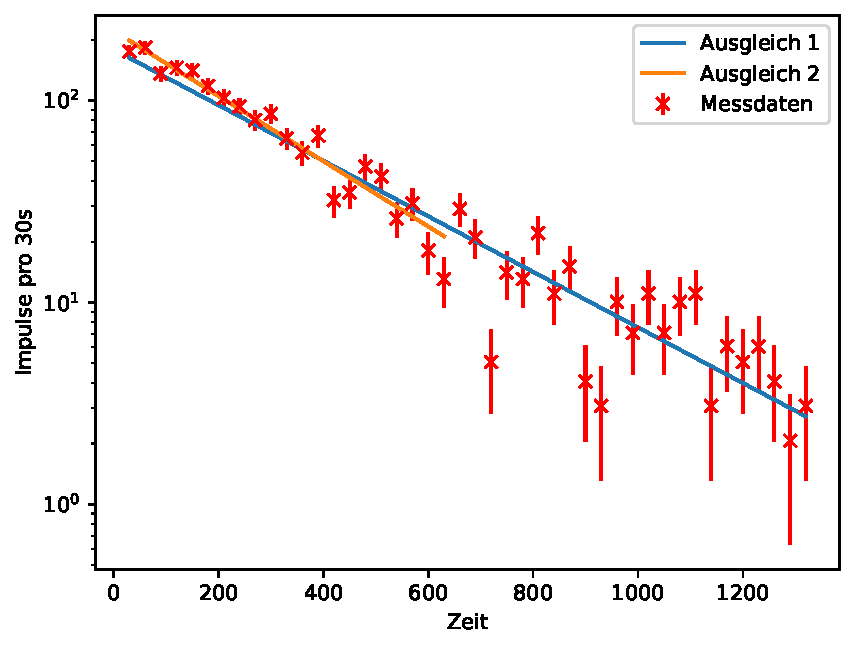
\includegraphics[width=0.7\textwidth]{plots/Vanadium.pdf}
    \caption{Ein sehr sehr toller Plot.}
\end{figure}
Mit \ref{eqn:Zerfallsgesetz} wird nun ein linearer Ausgleich gefertigt. \\
Für den blauen ''Ausgleich 1'' ergibt sich:
\begin{align*}
    \ln(N(t)) = m \cdot t + b\\
     m = -0.00317 \pm 0.00016 && b = 5.19 \pm 0.13 \\
    \lambda = -m = 0.00317 \pm 0.00016 \\
    T = \ln\left( \frac{2}{\lambda} \right) = 219 \pm 11 \text{s}
\end{align*}
Und für den orangenen ''Ausgleich 2'' mit gleicher Funktion:
\begin{align*}
     m = -0.00372 \pm 0.00023 && b = 5.40 \pm 0.08 \\
    \lambda = -m = 0.00372 \pm 0.00023 \\
    T = \ln\left( \frac{2}{\lambda} \right) = 186 \pm 11 \text{s}
\end{align*}

\subsection{Rhodium}
Auch für die Messwerte des Rhodium zerfalls muss die Nullrate herausgerechnet werden.
Dazu wird selbige wieder an das Intervall, in diesem Fall 15 Sekunden, angepasst.
\begin{align*}
    N_{\text{U},\text{Rhodium}} =  \frac{N_{\text{U}}}{20} = 6.96 \pm 0.22 \; \frac{\text{Imp}}{30\text{s}}
\end{align*}
\begin{figure}
    \centering
    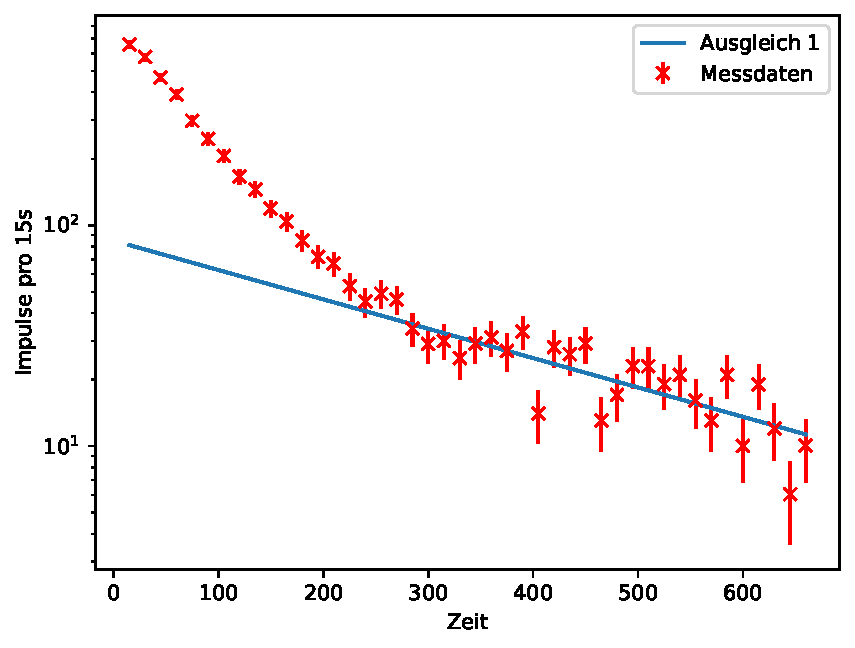
\includegraphics[width=0.7\textwidth]{plots/Rhodium_lang.pdf}
    \caption{Ein auch sehr toller Plot von Rhodium lang.}
\end{figure}
Aus dem Ausgleich ergibt sich für den langsamen Zerfall:
\begin{align*}
    \ln(N(t)) = m \cdot t + b\\
     m = -0.0031 \pm 0.0006 && b = 4.44 \pm 0.31 \\
    \lambda = -m = 0.0031 \pm 0.0006 \\
    T = \ln\left( \frac{2}{\lambda} \right) =  230 \pm 50 \text{s}
\end{align*}
\begin{figure}
    \centering
    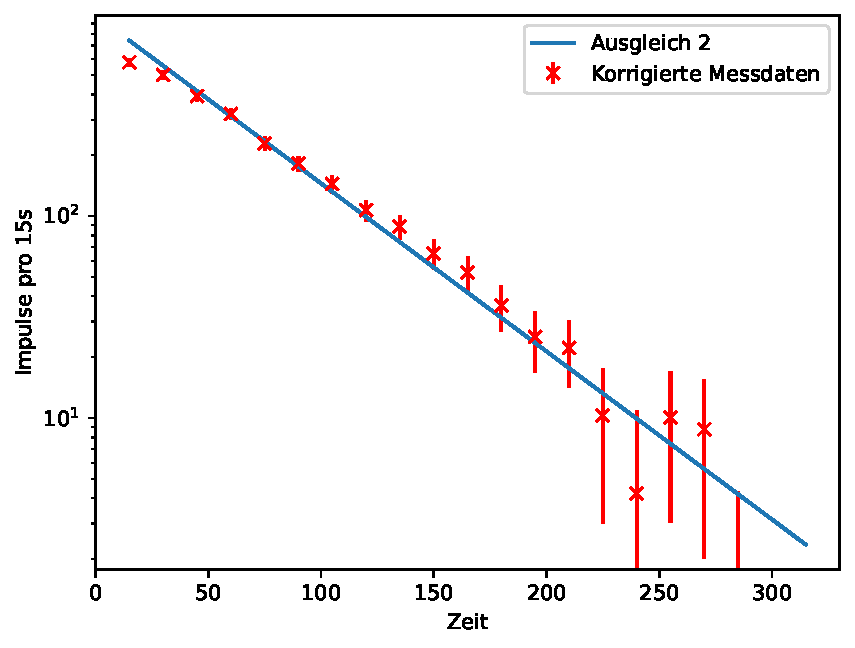
\includegraphics[width=0.7\textwidth]{plots/Rhodium_kurz.pdf}
    \caption{Ein super toller und netter Plot von rhodium kurz.}
\end{figure}
\begin{align*}
     m = -0.0192 \pm 0.0009 && b = 6.89 \pm 0.14 \\
    \lambda = -m = 0.0192 \pm 0.0009 \\
    T = \ln\left( \frac{2}{\lambda} \right) = 36.2 \pm 1.7 \text{s}
\end{align*}